\documentclass[hyperref={colorlinks, linkcolor=white, urlcolor=green!50!black}]{beamer}

%POZN.: Shrnout Assassin's Creed do jedné prezentace je celkem nemožné, proto jsem se zaměřil hlavně na postavy.

\usepackage[czech]{babel}
\usepackage[utf8]{inputenc}
\usepackage{bookman}
\usepackage{booktabs}
\usepackage{caption}
\usepackage{color}
\usepackage{float}
\usepackage{graphicx}
\usepackage{multicol}


\definecolor{darkred}{rgb}{0.8,0,0}
\definecolor{blendedblue}{rgb}{0.2,0.2,0.7}

\mode<presentation> {
	\usetheme{Rochester}
	\setbeamercolor{normal text}{fg=white,bg=black!95}
	\setbeamercolor{structure}{fg=darkred}
	\setbeamercolor{block title}{bg=blendedblue}
	\setbeamertemplate{caption}[numbered]
	\setbeamertemplate{footline}[frame number]
	\setbeamertemplate{navigation symbols}{}
}

\graphicspath{ {./img/} }


\title[Assassin's Creed]{\textbf{Assassin's Creed}} % The short title appears at the bottom of every slide, the full title is only on the title page
\subtitle{Nic není pravda. Vše je dovoleno.}
\author{Jakub Frýz}
\institute[VUT-FIT]{\textsc{Vysoké učení technické v~Brně} \\ \smallskip Fakulta informačních technologií}
\date{\today}

\begin{document}

\begin{frame}
	\titlepage
\end{frame}

\section{Obsah}

\begin{frame}
\frametitle{Obsah prezentace}
	\begin{multicols}{2}
		\tableofcontents
	\end{multicols}
\end{frame}

\section{Co je Assassin's Creed?}

\subsection{O~Assassin's Creed}

\begin{frame}
\frametitle{O~Assassin's Creed}
\begin{itemize}
	\item \textbf{\color{darkred} Assassin's Creed} je herní série od francouzké herní společnosti \textbf{\color{blendedblue} Ubisoft}, která si získala přízeň po celém světě.
	\item Zápletkou hry je prastarý boj mezi \textbf{\color{blendedblue} Bratrstvem asasínů} a \textbf{\color{blendedblue} Řádem templářů}.
	\item Tyto dvě skupiny mají stejný cíl a to \textbf{\color{green!50!black} mír na~zemi a~ve~všem}. Problémem však je, jak se toho snaží dosáhnout. Asasíni chtějí svobodnou mysl, zatímco templáři chtějí mysl ovládnout a podmanit si ji své vůli.
\end{itemize}

\end{frame}

\begin{frame}
\frametitle{O~Assassin's Creed}
\framesubtitle{pokračování}
\begin{columns}[c]
	
	\column{.6\textwidth}
	\begin{itemize}
		\item K~tomu jim mohou dopomoci \textbf{\color{green!50!black} kousky~Ráje}, předměty nesmírné moci, které zde zanechala \textbf{\color{darkred} První civilizace}.
		\item Asasíni se snaží tyto kousky Ráje najít dřív, aby tak zabránili templářům ovládnout svět, i kdyby se měli navzájem pozabíjet.
	\end{itemize}
	
	\column{.4\textwidth}
	\begin{figure}[h]
		\centering
		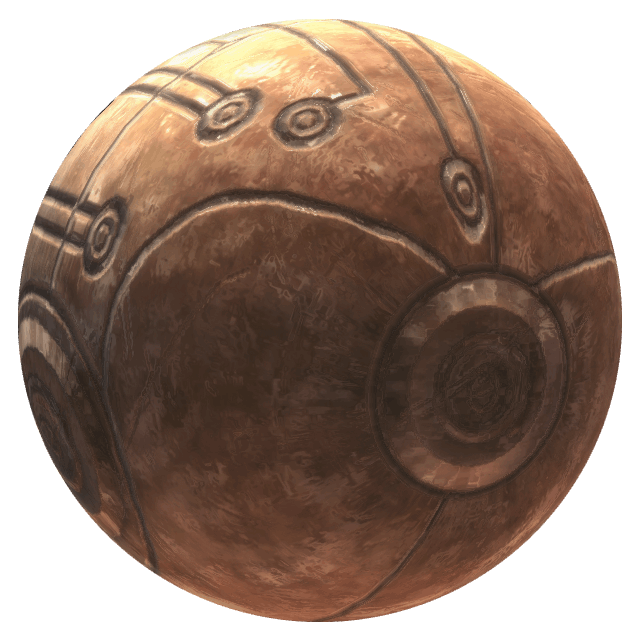
\includegraphics[width=\textwidth]{item_apple}
		\captionsetup{labelformat=empty, justification=centering}
		\caption{\textbf{\color{blendedblue} Jablko Ráje} \\ jeden z~kousků Ráje}
	\end{figure}
	
\end{columns}

\end{frame}

\begin{frame}
\frametitle{O~Assassin's Creed}
\framesubtitle{pokračování}
\begin{itemize}
	\item Ve~hře se dostanete do~kůže jednoho z~asasínů a~máte tak možnost prožít část jeho života, likvidovat templáře, hledat kousky Ráje, poklady\dots .
	\item Hra je zasazena do~naší historie, takže zde můžete potkat i~takové postavy jako je {\color{darkred} Leonardo da~Vinci}, {\color{darkred} Napoleon Bonaparte}, {\color{darkred} královna Viktorie}, aj..
\end{itemize}

\end{frame}

\subsection{Znaky}

\begin{frame}
\frametitle{Znaky}
\begin{columns}[c]
	
	\column{.5\textwidth}
	\begin{figure}[ht]
		
\includegraphics[height=150px]{logo_assassins}
		\captionsetup{labelformat=empty}		
		\caption{Bratrstvo asasínů}
	\end{figure}
	
	\column{.5\textwidth}
	\begin{figure}[ht]
		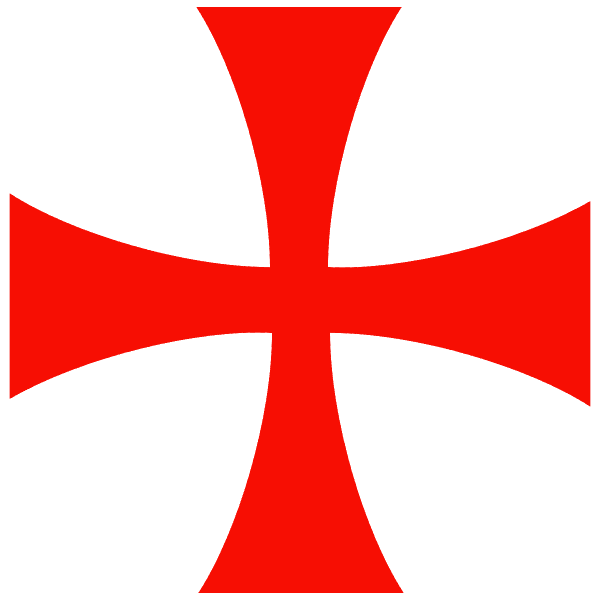
\includegraphics[height=150px]{logo_templars}
		\captionsetup{labelformat=empty}
		\caption{Řád templářů}
	\end{figure}
	
\end{columns}
\end{frame}

\section{Důležité postavy}

\subsection[Altair]{Altaïr Ibn-La'Ahad}

\begin{frame}\label{altair}
\frametitle{Altaïr Ibn-La'Ahad}
\framesubtitle{(1165 -- 1257) \hfill Assassin's Creed (2008)}
\begin{columns}[c]
	
	\column{.6\textwidth}
	\begin{block}{Info}
	\begin{itemize}
		\item kvůli své~aroganci byl zbaven postavení mistra asasína
		\item postavení si znovu získal zabitím devíti významných templářů ve~Svaté zemi a~navrácením Jablka do~rukou asasínů
		\item nakonec zrazen mentorem, kterého zabil
		\item mentor a~otec novodobých asasínů
		\item sepsal kodex
	\end{itemize}
	\end{block}
	
	\column{.4\textwidth}
	\begin{figure}[h]
		\centering
		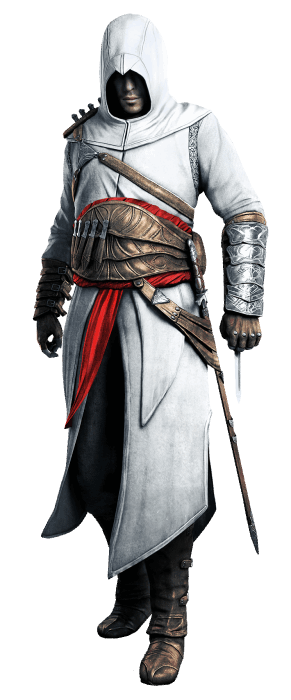
\includegraphics[height=200px]{char_altair}
	\end{figure}
	
\end{columns}
\end{frame}

\subsection[Ezio]{Ezio Auditore da Firenze}

\begin{frame}\label{ezio}
\frametitle{Ezio Auditore da Firenze}
\framesubtitle{(1459-1524) \hfill Assassin's Creed II (2010), Bratrstvo (2011), Odhalení (2011)}
\begin{columns}[c]

	\column{.4\textwidth}
	\begin{figure}[h]
		\centering
		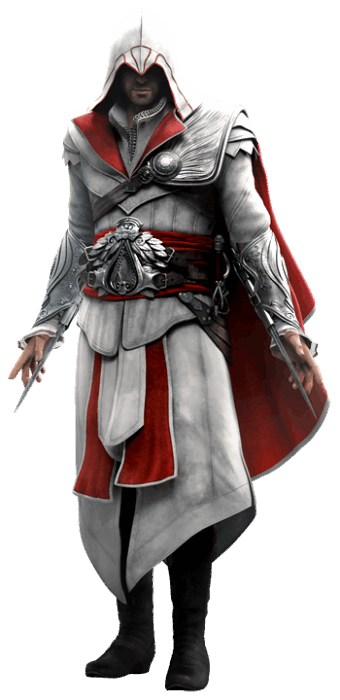
\includegraphics[height=200px]{char_ezio}
	\end{figure}
	
	\column{.6\textwidth}
	\begin{block}{Info}
	\begin{itemize}
		\item asasín v~Itálii za~dob renesance
		\item navrátil bratrstvu zašlou slávu
		\item celá jeho rodina, až~na~matku a~sestru, byla veřejně popravena z~křivého obvinění
		\item značnou část života bojoval proti rodině Borgiů, kteří byli templáři (Rodrigo a Cesare byli i velmistry)
		\item přítel s~{\color{darkred} Leonardem da Vinci}
	\end{itemize}
	\end{block}
	
\end{columns}
\end{frame}

\subsection[Connor]{Connor Kenway}

\begin{frame}\label{connor}
\frametitle{Connor Kenway (Ratonhnhaké:ton)}
\framesubtitle{(1756-\textit{unknown}) \hfill Assassin's Creed III (2012), Liberation (2014)}
\begin{columns}[c]
	
	\column{.6\textwidth}
	\begin{block}{Info}
	\begin{itemize}
		\item asasín v~Americe za~doby války o~nezávislost
		\item syn Haythama [\ref{haytham}] a~indiánky~Kaniehtí:io
		\item k~asasínům se přidal po~tom, co mu templáři vypálili vesnici jeho~kmene
		\item obnovil asasíny v~Americe
		\item ve~válce o~nezávislost Ameriky bojoval po~boku {\color{darkred} George Washingtona}
	\end{itemize}
	\end{block}
	
	\column{.4\textwidth}
	\begin{figure}[h]
		\centering
		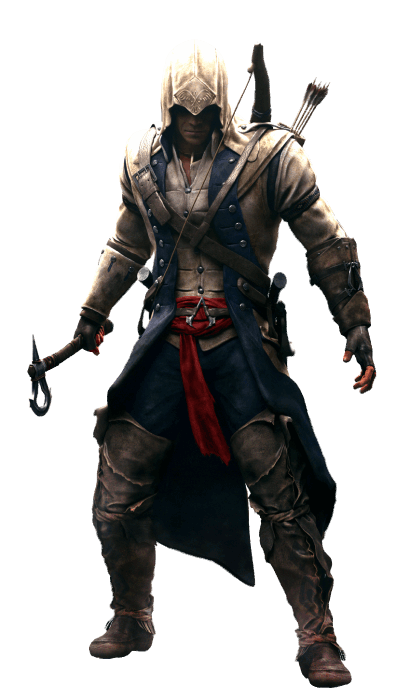
\includegraphics[height=200px]{char_connor}
	\end{figure}
	
\end{columns}
\end{frame}

\subsection[Haytham]{Haytham Kenway}

\begin{frame}\label{haytham}
\frametitle{Haytham Kenway}
\framesubtitle{(1725-1781) \hfill Assassin's Creed III (2012), Rogue (2014)}
\begin{columns}[c]

	\column{.4\textwidth}
	\begin{figure}[h]
		\centering
		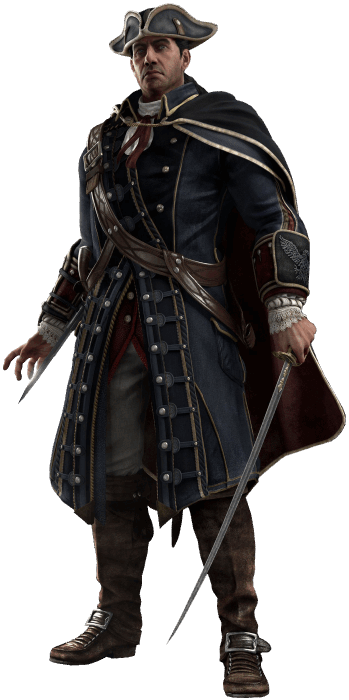
\includegraphics[height=200px]{char_haytham}
	\end{figure}
	
	\column{.6\textwidth}
	\begin{block}{Info}
		\begin{itemize}
			\item syn Edwarda [\ref{edward}]
			\item po~vraždě otce vycvičen jako templář vrahem svého otce (aniž by měl o~tom ponětí)
			\item nakonec se stal velmistrem templářů
			\item zabit synem Connorem [\ref{connor}]
		\end{itemize}
	\end{block}

\end{columns}
\end{frame}

\subsection[Shay]{Shay Cormac}

\begin{frame}\label{shay}
\frametitle{Shay Cormac}
\framesubtitle{(1731-\textit{unknown}) \hfill Assassin's Creed Rogue (2014)}
\begin{columns}[c]
	
	\column{.6\textwidth}
	\begin{block}{Info}
		\begin{itemize}
			\item bývalý asasín, přidal se k~templářům
			\item asasíny zradil z~důvodu, že se mu nelíbili jejich praktiky
			\item z~velké části zničil asasíny v~Americe
			\item získal mnohé kousky Ráje pro~templáře
			\item v~r. 1766 ve~Versailles zabil asasína Charlese Doriana, otce Arna [\ref{arno}]
		\end{itemize}
	\end{block}
	
	\column{.4\textwidth}
	\begin{figure}[h]
		\centering
		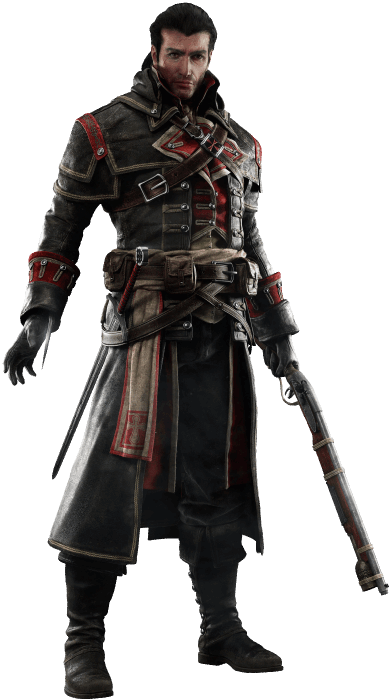
\includegraphics[height=200px]{char_shay}
	\end{figure}
	
\end{columns}
\end{frame}

\subsection[Edward]{Edward Kenway}

\begin{frame}\label{edward}
\frametitle{Edward James Kenway}
\framesubtitle{(1693-1735) \hfill Assassin's Creed IV Black Flag (2013)}
\begin{columns}[c]
	
	\column{.4\textwidth}
	\begin{figure}[h]
		\centering
		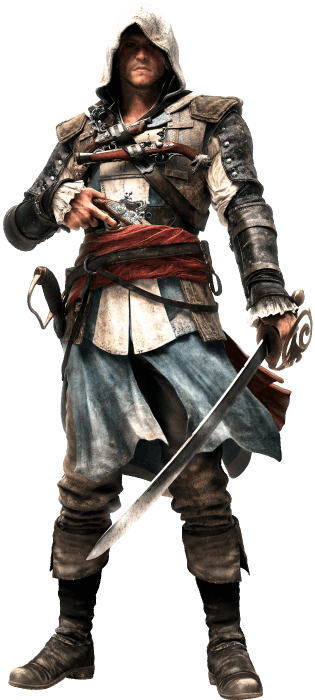
\includegraphics[height=200px]{char_edward}
	\end{figure}
	
	\column{.6\textwidth}
	\begin{block}{Info}
	\begin{itemize}
		\item bukanýr, později pirát a~nakonec i~asasín, v~karibských vodách
		\item ochránil Observatoř před~zneužitím templáři
		\item nakonec se usadil v~Londýně
		\item zavražděn přítelem, ze~kterého se vyklubal templář
		\item na vodách se plul i~se~známými piráty jako je např. {\color{darkred} Černovous}, {\color{darkred} James Kidd}, aj.
	\end{itemize}
	\end{block}
	
\end{columns}
\end{frame}

\subsection[Arno]{Arno Dorian}

\begin{frame}\label{arno}
\frametitle{Arno Victor Dorian}
\framesubtitle{(1768-\textit{unknown}) \hfill Assassin's Creed Unity (2014)}
\begin{columns}[c]
	
	\column{.6\textwidth}
	\begin{block}{Info}
	\begin{itemize}
		\item asasín v~Paříži během francouzské revoluce
		\item po~vraždě otce vychováván velmistrem templářů
		\item velmistr byl v~r.\,1789 zavražděn někým z~řádu a~vina padla na~Arna
		\item uvězněn v~Bastille se dozvídá o~svém~asasínském původu
		\item později zjišťuje totožnost a~intriky vraha velmistra, nakonec jej i~zabije
	\end{itemize}
	\end{block}
	
	\column{.4\textwidth}
	\begin{figure}[h]
		\centering
		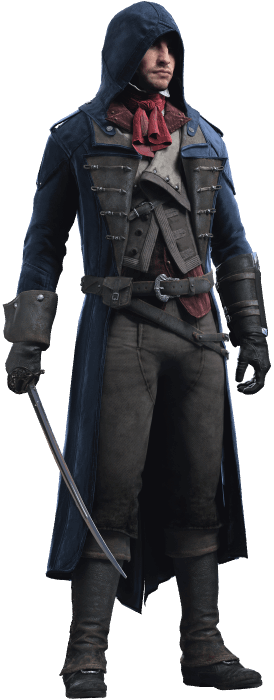
\includegraphics[height=200px]{char_arno}
	\end{figure}
	
\end{columns}
\end{frame}

\subsection[Jacob, Evie]{Jacob \& Evie Frye}

\begin{frame}\label{jacob,evie}
\frametitle{Jacob \& Evie Frye}
\framesubtitle{(1847-\textit{unknown}) \hfill Assassin's Creed Syndicate (2015)}
\begin{columns}[c]
	
	\column{.4\textwidth}
	\begin{figure}[h]
		\centering
%		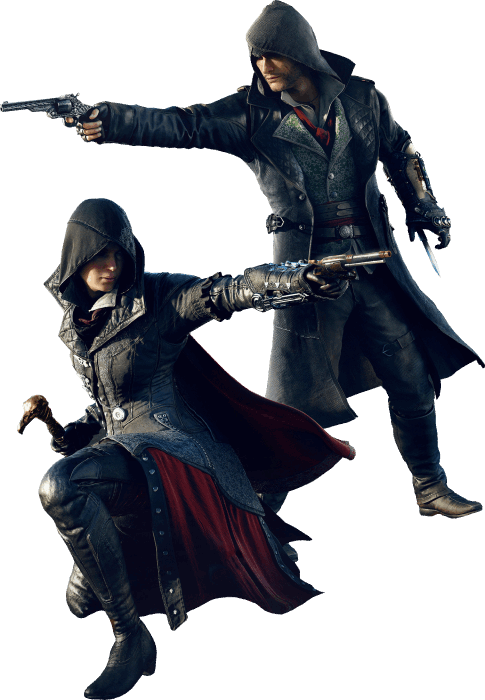
\includegraphics[height=200px]{char_twins}
		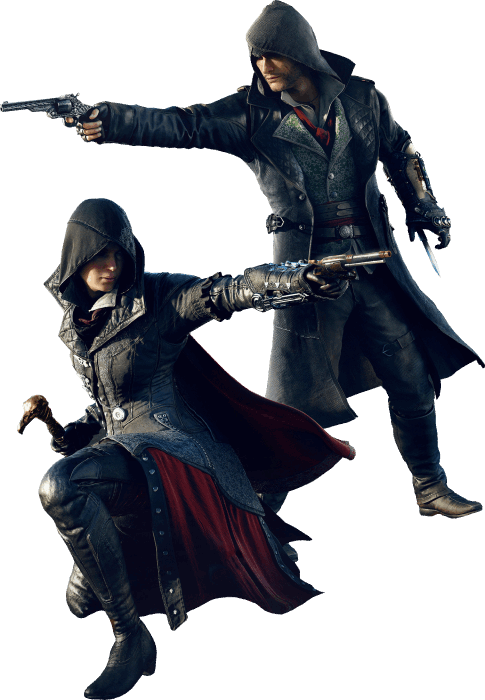
\includegraphics[width=\textwidth]{char_twins}
	\end{figure}

	\column{.6\textwidth}
	\begin{block}{Info}
		\begin{itemize}
			\item dvojčata asasíni v~Londýně v~době průmyslové revoluce
			\item zatímco Jacob vedl gang, kterým destabilizovával templáře v~Londýně, Evie hledala zmínky o~artefaktu, který měli templáři ve~vlastnictví
			\item po zničení templářů v~Londýně je královna Viktorie povýšila do rytířského stavu
		\end{itemize}
	\end{block}
	
\end{columns}
\end{frame}

\section{Na závěr}

\begin{frame}
\frametitle{Na závěr}
\begin{alertblock}{Důvod výběru}
	Assassin's Creed je jedna z~mých nejvíce oblíbených herních sérií, se kterou jsem strávil spoustu času, ať už u~počítače nebo s~knížkami a komiksy, které příběh her doplňují.
\end{alertblock}
\begin{block}{Text v~prezentaci}
	Většina textu byla napsána z~vlastní hlavy, a proto v~něm mohou být menší odchylky či chyby. %kdybych si toho tolik pamatoval z jakéhokoliv předmětu
\end{block}
\begin{exampleblock}{Použité zdroje}
	Všechny obrázky použité v~této prezentaci byly staženy z~webu \href{http://assassinscreed.wikia.com}{assassinscreed.wikia.com}.
\end{exampleblock}
\end{frame}

\section{Konec}

\begin{frame}
\frametitle{\hspace*{\fill} \textbf{\textsc{Nic není pravda. Vše je dovoleno.}} \hspace*{\fill}}

\includegraphics[width=\textwidth]{logo_ac_white}
\end{frame}

\end{document}